%---------------------------------------------------------------------------------------
% Propuesta de solución
%
%---------------------------------------------------------------------------------------
\DocumentMetadata{lang=es-MX}
\documentclass[stu,12pt,floatsintext,draftfirst,spanish]{report}

%-----------------------------------------PAQUETES--------------------------------------
\usepackage[spanish,mexico]{babel}
\usepackage[utf8]{inputenc}
\usepackage{times}
\usepackage{physics,amsmath,amssymb,siunitx,codehigh,cancel,float}
\usepackage{hyperref}
\usepackage{csquotes,ragged2e}
\usepackage{tabularray}
\UseTblrLibrary{booktabs}
\usepackage[x11names]{xcolor}
\usepackage{graphicx}
\usepackage[style=apa,sortcites=true,sorting=nyt,backend=biber]{biblatex}
%\addbibresource{referencias.bib}

\DeclareLanguageMapping{spanish}{spanish-apa}

%-------------------------------ESPECIFICACIONES DEL PDF--------------------------------
\hypersetup{
colorlinks=false,
pdfhighlight=/O,
pdfauthor={Jocelyn Janet Parés Ramos},
pdftitle={Propuesta de},
pdfsubject={ASUNTO DEL PDF},
pdfkeywords={PALABRAS CLAVE},
pdfproducer={LaTeX con hyperref},
pdfcreator={pdfLaTeX},
pdfstartview={Fit},
pdfpagemode={UseOutlines},
pdfnewwindow=true,
pdfpagetransition= R,
pdflang=es-MX,
}

%PORTADA--------------------------------------------------------------------------------
\title{Propuesta de solución}
\author{Jocelyn Janet Parés Ramos & 
        Juan Pablo de la Vega Lozano &
        Carlos Alberto Torre Sánchez &
        Ana Camila Murillo Fernández &
        Gael García Zúñiga}
\date{11 de abril, 2025}



%-----------------------------------------DOCUMENTO-----------------------------------------
\begin{document}
\maketitle 

El problema que pensamos resolver es el [\dots.]
 
Nuestra estrategia para resolver el problema es el modelar el sistema de John Deere con el modelo HX10 con 2 cuchillas. Primero, se debe de hacer un análisis de la situación actual del sistema, para después hacer un análisis de los parámetros que se tienen que considerar para el modelo. Las cuchillas funcionan de la siguiente manera:
\begin{figure}[htbp]
    \centering
    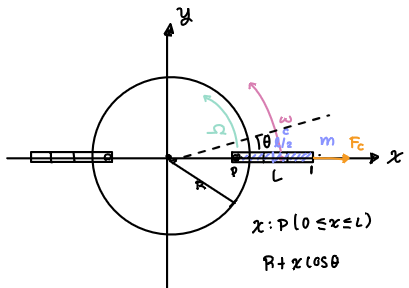
\includegraphics[width=0.5\textwidth]{diagrama.png}
    \caption{Diagrama de nuestro modelo.}
    \label{<label>}
\end{figure}

Queremos encontar una función de $\theta$. Primero tenemos las siguientes variables:
- $L$: La longitud de la cuchilla
- $m$: La masa de la cuchilla
- $R$: El radio del círculo
- $P$: El punto en donde la cuchilla oscila con respecto al eje
- $\Omega$: La velocidad angular del disco
- $b$: El coeficiente de amortiguamiento (proporcional a la velocidad angular y la rotación del disco)

$$
\sum \tau = I \alpha 
$$

Primero encontramos el momento de incercia total, para esto sería obtener el momento de la cuchilla y el del círculo. Para una varilla el momento de incercia se define como:

$$
I= \int_{\frac{-L}{2}}^{\frac{L}{2}}r^{2} \frac{M}{L}dr= \frac{M}{L} \frac{r^{3}}{3} \Big|

%REFERENCIAS----------------------------------------------------------------------------

%\printbibliography

\end{document}

